\appendix                               %imposta le appendici
\chapter{Rette di calibrazione dei TDC}               %crea l'appendice
Vengono di seguito riportate le rette di calibrazione del Time to Digital Converter.

\begin{figure}[H]
  \centering
  \subfloat[][]{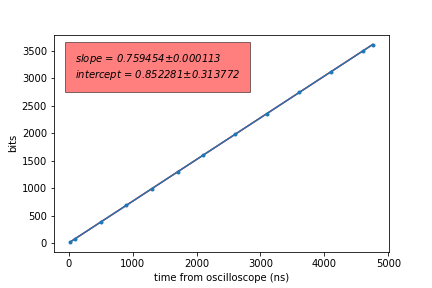
\includegraphics[width=.4\textwidth]{plots/tdc11.png}\label{tdc11}}\quad
  \subfloat[][]{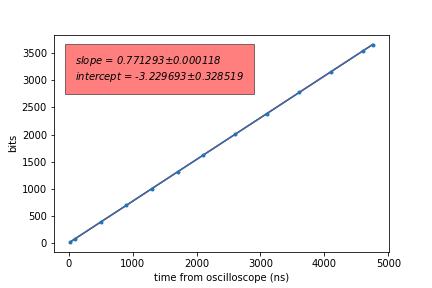
\includegraphics[width=.4\textwidth]{plots/tdc12.png}\label{tdc12}}\\
  \subfloat[][]{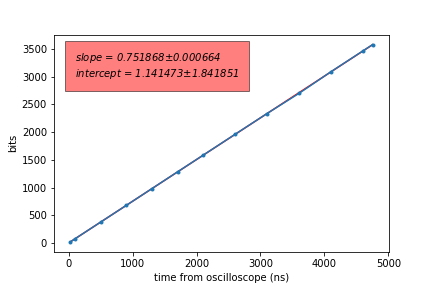
\includegraphics[width=.4\textwidth]{plots/tdc13.png}\label{tdc13}}\quad
  \subfloat[][]{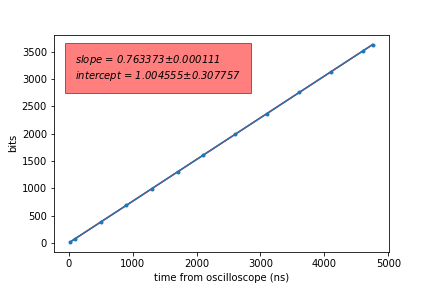
\includegraphics[width=.4\textwidth]{plots/tdc14.png}\label{tdc14}}\\
  \subfloat[][]{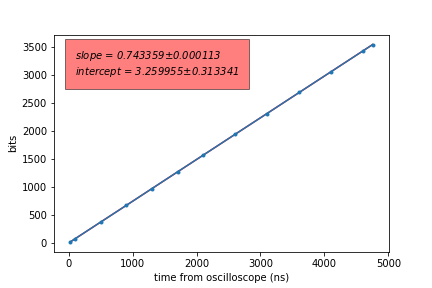
\includegraphics[width=.4\textwidth]{plots/tdc15.png}\label{tdc15}}\quad
  \subfloat[][]{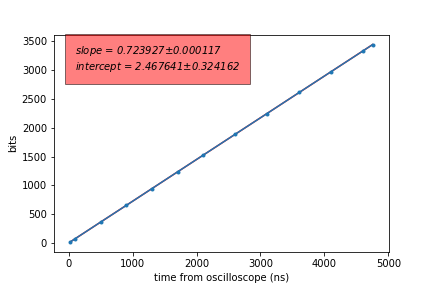
\includegraphics[width=.4\textwidth]{plots/tdc16.png}\label{tdc16}}\\
  \subfloat[][]{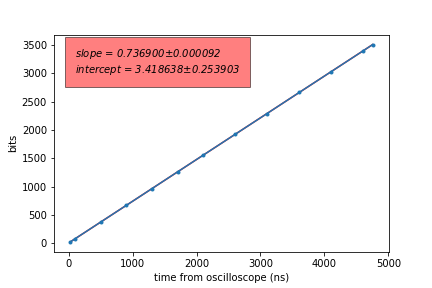
\includegraphics[width=.4\textwidth]{plots/tdc17.png}\label{tdc17}}\quad
  \subfloat[][]{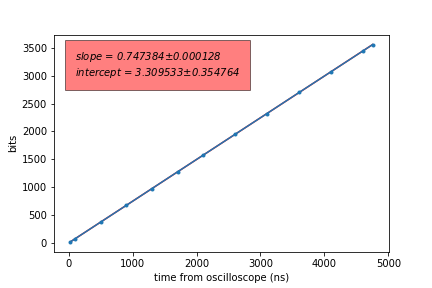
\includegraphics[width=.4\textwidth]{plots/tdc18.png}\label{tdc18}}\\
  \caption{}
  \label{fig:tdc1}
\end{figure}

\begin{figure}[H]
  \centering
  \subfloat[][]{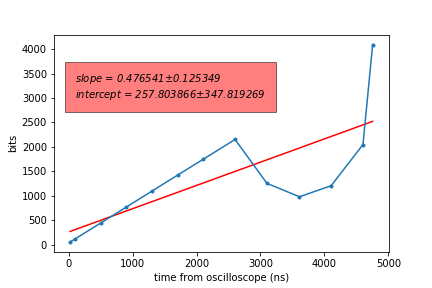
\includegraphics[width=.4\textwidth]{plots/tdc21.png}\label{tdc21}}\quad
  \subfloat[][]{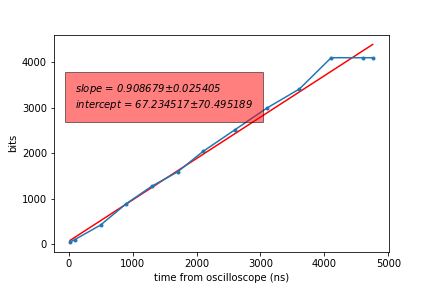
\includegraphics[width=.4\textwidth]{plots/tdc22.png}\label{tdc22}}\\
  \subfloat[][]{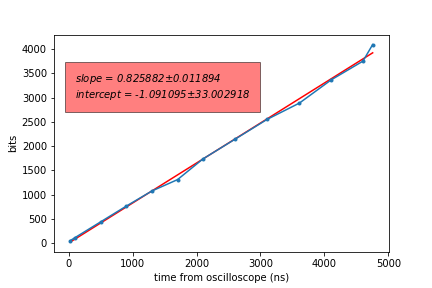
\includegraphics[width=.4\textwidth]{plots/tdc23.png}\label{tdc23}}\quad
  \subfloat[][]{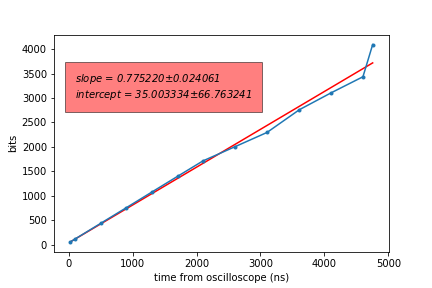
\includegraphics[width=.4\textwidth]{plots/tdc24.png}\label{tdc24}}\\
  \subfloat[][]{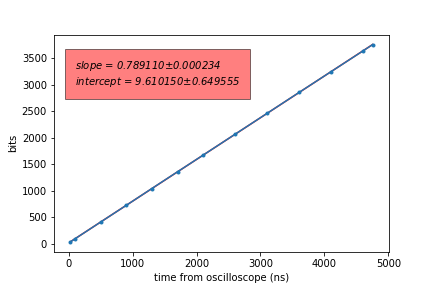
\includegraphics[width=.4\textwidth]{plots/tdc25.png}\label{tdc25}}\quad
  \subfloat[][]{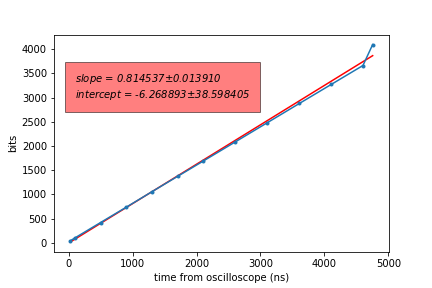
\includegraphics[width=.4\textwidth]{plots/tdc26.png}\label{tdc26}}\\
  \subfloat[][]{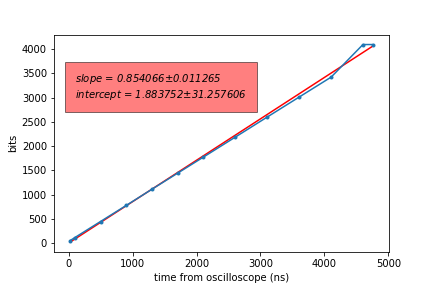
\includegraphics[width=.4\textwidth]{plots/tdc27.png}\label{tdc27}}\quad
  \subfloat[][]{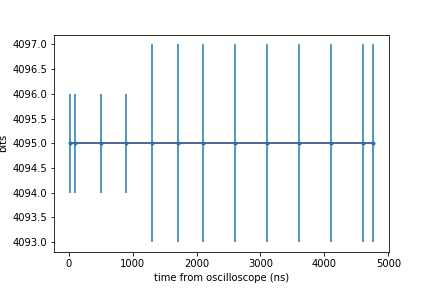
\includegraphics[width=.4\textwidth]{plots/tdc28.png}\label{tdc28}}\\
  \caption{}
  \label{fig:tdc2}
\end{figure}








\rhead[\fancyplain{}{\bfseries \thechapter \:Prima Appendice}]
{\fancyplain{}{\bfseries\thepage}}








\chapter{Seconda Appendice}             %crea l'appendice
%%%%%%%%%%%%%%%%%%%%%%%%%%%%%%%%%%%%%%%%%imposta l'intestazione di pagina
\rhead[\fancyplain{}{\bfseries \thechapter \:Seconda Appendice}]
{\fancyplain{}{\bfseries\thepage}}









































\begin{thebibliography}{90}             %crea l'ambiente bibliografia
\rhead[\fancyplain{}{\bfseries \leftmark}]{\fancyplain{}{\bfseries
\thepage}}
%%%%%%%%%%%%%%%%%%%%%%%%%%%%%%%%%%%%%%%%%aggiunge la voce Bibliografia
                                        %   nell'indice
\addcontentsline{toc}{chapter}{Bibliografia}
%%%%%%%%%%%%%%%%%%%%%%%%%%%%%%%%%%%%%%%%%provare anche questo comando:
%%%%%%%%%%%\addcontentsline{toc}{chapter}{\numberline{}{Bibliografia}}
\bibitem{pdg} M. Tanabashi et al. (Particle Data Group), Phys. Rev. D 98, 030001 (2018).
\bibitem{K2} Secondo oggetto bibliografia.
\bibitem{K3} Terzo oggetto bibliografia.
\bibitem{K4} Quarto oggetto bibliografia.
\end{thebibliography}
%%%%%%%%%%%%%%%%%%%%%%%%%%%%%%%%%%%%%%%%%non numera l'ultima pagina sinistra

